\documentclass[a4paper,12pt]{article}
\usepackage[utf8]{inputenc}
\usepackage{calc}
\usepackage{eso-pic}
\usepackage{graphicx}
\usepackage{parskip}
\usepackage{hyperref}
\usepackage[a4paper,left=25 mm,right=25 mm, bottom=25 mm,
    margin=1in,top=25 mm]{geometry} % Adjusting the margins
\usepackage{tikz}
\usepackage{array}
\usepackage{pdfpages}
\usepackage{tabularx}
\usepackage{amsmath}
\usepackage{amssymb}
\usepackage{paralist}
\usepackage{ragged2e}
\usetikzlibrary{calc}

\begin{document}

\begin{titlepage}
\begin{tikzpicture}
    [remember picture, overlay]
    \draw[line width = 2pt, black] 
        ($(current page.north west) + (1cm,-1cm)$) 
        rectangle 
        ($(current page.south east) + (-1cm,1cm)$);
\end{tikzpicture}
    \centering
    \vspace*{0 cm}
    \LARGE
    \textbf{Maulana Abul Kalam Azad University of Technology, WB}
    \vspace{0.5cm}
    
    
\includegraphics[width=0.3\textwidth]{makaut1.png} % Assuming you have the logo image
    \vspace{0.5cm}
    
    \Large
    \textbf{\textcolor{blue!60}{Software Tools and Technology\\
        -: Lab Notebook :-}}
    \vspace{0.5cm}
    
    \large
    \textbf{\textcolor{red}{Group 11}}
    \vspace{0.5 cm}
    
    \textbf{Repository Link:} \href{https://github.com/Rajarshi-2005/LaTeX-Group-11}{https://github.com/Rajarshi-2005/LaTeX-Group-11}
    \vspace{0.5cm}
    
    \textbf{\underline{\textcolor{blue!60}{Group Members}}}
    \vspace{0.4cm}

    \normalsize
    \begin{enumerate}
        \item \textbf{Rajarshi Biswas}\\
              \textbf{Roll No: 30085323005}\\
              \textbf{Department: BSc in IT (Cyber Security)}
        \item \textbf{Agnik Dey}\\
              \textbf{Roll No: 30085323019}\\
              \textbf{Department: BSc in IT (Cyber Security)}
        \item \textbf{Aditi Ghosh}\\
              \textbf{Roll No: 30059223047}\\
              \textbf{Department: BSc in Forensic Science}
        \item \textbf{Nawazish Alam}\\
              \textbf{Roll No: 30084323041}\\
              \textbf{Department: BSc in IT (Data Science)}
              \item \textbf{Aabir Sengupta}\\
              \textbf{Roll No: 39959223039}\\
              \textbf{Department: BSc in Forensic Science}
    \end{enumerate}
    \vspace{0.5 cm}
    
    \textbf{Instructor:} \href{mailto:ayan.ghosh@university.edu}{\textcolor{blue}{Ayan Ghosh \text{\&} Pabitra Pal}}\\
    \textbf{\textit{Date: September 11, 2024}}

\end{titlepage}
\newpage
\begin{tikzpicture}
    [remember picture, overlay]
    \draw[line width = 2pt, black]
        ($(current page.north west) + (1cm,-1cm)$)
        rectangle 
        ($(current page.south east) + (-1cm,1cm)$);
\end{tikzpicture}
\vspace{-2cm}

\centering
\section*{\underline{\Huge\textbf{\textcolor{blue!60}{Index}}}}
\vspace{0.5cm}

\renewcommand{\arraystretch}{2}
\setlength{\tabcolsep}{0pt} 

\begin{tabular}{|>{\centering\arraybackslash}p{50pt}|>{\centering\arraybackslash}p{350pt}|>{\centering\arraybackslash}p{80pt}|}
\hline
\textbf{Serial No.} & \textbf{Questions} & \textbf{Sign}\\
\hline
1 & Introduction to GitHub and GitHub Desktop version installation  &\\\hline
2 & Building a C program for a calculator in the local repository,committing,and publishing it as a public repository &\\\hline
3 & Converting a submit button to Chin Tapak Dum Dum &\\\hline
4 & Branching and Merging &\\\hline
5 & Introduction to LaTeX and LaTeX installation&\\\hline
6 & Make a CV using LaTeX &\\\hline
\end{tabular}

\newpage
\begin{tikzpicture}
    [remember picture, overlay]
    \draw[line width = 2pt, black] 
        ($(current page.north west) + (1cm,-1cm)$) 
        rectangle 
        ($(current page.south east) + (-1cm,1cm)$);
\end{tikzpicture}
\vspace{-2cm}

\section*{\Huge{\textcolor{blue!60}{\underline{Lab Notebook Entries}}}}
\subsection*{Entry by: Rajarshi Biswas}
\textit{Date: [\today]}
\vspace{1 cm}
\begin{figure}[h!]
   \centering
    
\includegraphics[width=0.5\linewidth]{OIP.jpeg}
\end{figure}
\vspace{0.5 cm}

\section*{\Huge{\underline{{-:GitHub:-}}}}
\paragraph{}{GitHub is a web-based platform that allows developers to host, share, and collaborate on software projects. It provides a version control system powered by Git, enabling teams to track changes, manage code repositories, and work together seamlessly across different locations. GitHub supports collaborative development through features like pull requests, issues, and project boards, making it essential for open-source projects and professional software development. Additionally, it integrates with various development tools, enhancing productivity and streamlining the software development lifecycle.}

\subsection*{\underline{-:Installation:-}}
\paragraph{}{Installing GitHub Desktop is a straightforward process that enhances your workflow by providing a user-friendly interface for managing repositories. To begin, download the installer from the [official GitHub Desktop website](https://desktop.github.com/) for your operating system—Windows or macOS. After downloading, run the installer and follow the on-screen instructions to complete the setup. Once installed, launch the application and sign in with your GitHub credentials, or create a new account if needed. GitHub Desktop simplifies the process of cloning repositories, making commits, and managing branches, making it an invaluable tool for developers of all skill levels. For Linux users, alternative methods like using Wine or other Git clients are available.}


\newpage
\begin{tikzpicture}
    [remember picture, overlay]
    \draw[line width = 2pt, black] 
        ($(current page.north west) + (1cm,-1cm)$) 
        rectangle 
        ($(current page.south east) + (-1cm,1cm)$);
\end{tikzpicture}
\vspace{-2cm}
\subsection*{Entry by: Agnik Dey}
\textit{Date: [\today]}\\
\section*{\large{Git Assignment 2 : C program for calculator in the local
{\underline{repository and publishing it a public repository}}}}
\paragraph{}
The primary purpose of a calculator program is to perform mathematical calculations efficiently and accurately. It provides a user-friendly interface for entering numbers and operators, and then quickly calculates and displays the result. 

Calculators can range from simple devices that handle basic arithmetic to more advanced ones capable of complex functions like trigonometry, statistics, and even programming. They are widely used in various fields, including education, science, engineering, and everyday life.

\begin{center}
\section*{\underline{{:Explain the code properly:}}}
\end{center}

\paragraph{}
This C program is designed to function as a simple calculator, allowing users to perform basic arithmetic operations (addition, subtraction, multiplication, and division).\\

\begin{flushleft}
\underline{\textbf{Key Components and Their Functions:}}\\
\end{flushleft}

\begin{enumerate}

\item Header Inclusion:
   - $\text{\#}include <stdio.h>$ : This includes the standard input/output library, which provides functions like printf (for printing output) and scanf (for reading input).\\

\item  Main Function:
   - int main(): This is the entry point of the program. It's where the execution begins.\\

\item Variable Declarations:
   - char operator: Stores the operator entered by the user (+, -, *, /).
   - double num1, num2: Stores the two numbers entered by the user.
   - double result: Stores the calculated result.\\

\item User Input:
   - printf("Enter an operator (+, -, *, /): ");: Prompts the user to enter an operator.
   - scanf("%c", &operator);: Reads the character entered by the user and stores it in the operator variable.
   - Similar prompts and reads are used for the two numbers.\\

\item Operator Checking and Calculation:
   - switch (operator): This is a conditional statement that checks the value of the operator variable.
   - case `+':, case `-':, case `*':, case `/':: These cases handle different operators.
   - The respective arithmetic operations are performed based on the operator and the results are stored in the result variable.
   - A check for division by zero is included to prevent errors.\\

\item Output:
   - printf(``Result: ")\\
\end{enumerate}

\begin{flushleft}
    \underline{\textbf{Flow of Execution:}}\\
\end{flushleft}

\begin{enumerate}
\item{The program starts execution from the main function.}\\
\item The user is prompted to enter an operator.\\
\item The entered operator is stored.\\
\item The user is prompted to enter two numbers.\\
\item The entered numbers are stored.\\
\begin{tikzpicture}
    [remember picture, overlay]
    \draw[line width = 2pt, black] 
        ($(current page.north west) + (1cm,-1cm)$) 
        rectangle 
        ($(current page.south east) + (-1cm,1cm)$);
\end{tikzpicture}
\item The switch statement checks the operator and performs the corresponding calculation.\\
\item The result is printed.\\
\item The program ends.\\
\end{enumerate}

\paragraph{}
Overall, this code provides a basic calculator functionality by taking user input for operator and two numbers, performing the calculation based on the operator, and displaying the result.


\section*{\large{How to use it, what will be the output after program \underline{compilation, set an example}}}


\begin{flushleft}
    \underline{\textbf{How to Use:}}
\end{flushleft}

\begin{enumerate}

\item Compile the code:
   - Save the code in a .c file (e.g., calculator.c).
   - Open a terminal or command prompt.
   - Navigate to the directory where you saved the file.
   - Compile the code using a C compiler like GCC:
     gcc calculator.c -o calculator
     This will create an executable file named calculator.\\

\item Run the program:
   - Execute the executable file:
     ./calculator

Example:\\
Enter an operator (+, -, *, /): +\\
Enter two numbers: 5 3\\
Result: 8.00\\

In this example:
- The user enters + as the operator.\\
- The user enters 5 and 3 as the numbers.\\
- The program calculates 5 + 3 and prints the result 8.00.\\

Other examples:\\
- - as the operator: 5 - 3 will result in 2.00.\\
- * as the operator: 5 * 3 will result in 15.00.\\
- / as the operator: 5 / 3 will result in 1.67.\\
\end{enumerate}
\vspace{0.5 cm}

\textbf{Calculator program link:} \href{https://github.com/Rajarshi-2005/calculator/blob/main/cal.c}{https://github.com/Rajarshi-2005/calculator/blob/main/cal.c}



\newpage
\begin{tikzpicture}
    [remember picture, overlay]
    \draw[line width = 2pt, black] 
        ($(current page.north west) + (1cm,-1cm)$) 
        rectangle 
        ($(current page.south east) + (-1cm,1cm)$);
\end{tikzpicture}
\vspace{-2cm}
\subsection*{Entry by: Aditi Ghosh}
\textit{Date: [\today]}\\
\section*{\large{Git Assignment 3 : Converting a submit button to Chin Tapak \underline{Dum Dum}}}
\paragraph{}
\begin{flushleft}
\text{\#}Steps to Fix the Button and Create a Pull Request:-\\
\end{flushleft}
\vspace{0.5 cm}
\begin{enumerate}
\item\textbf{Clone the Repository:}
   - You’ve already cloned the repository using GitHub Desktop, so you should have the project on your local machine.\\

\item\textbf{Open the Project:}
   - Open the project in your preferred IDE as per the instructions in the readme.md.\\

\item\textbf{Locate the Button Code:}
   - Search for the code where the submit button is defined. This is typically found in the frontend code of the application. Depending on the technology stack used (e.g., HTML/CSS, React, Angular, etc.), it could be in a file like index.html, App.js, ButtonComponent.js, or a similar file.\\

\item\textbf{Rename the Button:}
   - You renamed the button to ``Chin Tapak Dum Dum". If the button’s size became disproportionate, it’s likely due to styling issues.\\

\item\textbf{Test the Application:}
   - Run the application again to ensure that the button appears correctly and that there are no additional issues.\\

\item\textbf{Commit Your Changes:}
   - Once the button looks good, commit your changes. Use descriptive commit messages, for example: Fixed button styling after renaming.

   bash
   git add .
   git commit -m ``Fixed button styling after renaming to `Chin Tapak Dum Dum'"
   \\
   
\item\textbf{Push Your Changes:}
   - Push your changes to your forked repository on GitHub.

   bash
   git push origin main
   (Replace main with the correct branch name if it's different.)\\
   
\item\textbf{Create a Pull Request:}
   - Go to the original repository on GitHub (the one you cloned from).
   - You should see an option to create a pull request from your forked repository. Follow the instructions to create a pull request with a title and description of what you have done.

   Make sure to mention in the pull request that you have fixed the button styling after renaming it.
\end{enumerate}
\vspace{0.5 cm}

\textbf{Submit button link:} \href{https://github.com/Rajarshi-2005/STT/blob/main/SymbolApp.java}{https://github.com/Rajarshi-2005/STT/blob/main/SymbolApp.java}


\newpage
\begin{tikzpicture}
    [remember picture, overlay]
    \draw[line width = 2pt, black] 
        ($(current page.north west) + (1cm,-1cm)$) 
        rectangle 
        ($(current page.south east) + (-1cm,1cm)$);
\end{tikzpicture}
\vspace{-2cm}
\subsection*{Entry by: Nawazish Alam}
\textit{Date: [\today]}\\
\section*{\underline{{\LARGE{Git Assignment 4 : Branching and Merging}}}}

\paragraph{Objective:} Demonstrate proficiency in Git branching, merging, and conflict resolution.

\vspace{0.5cm}

% Manually resizing the images to fit within the page margins
% Screenshot 1
\begin{figure}[h!]
    \centering
     \hspace{4 cm}
     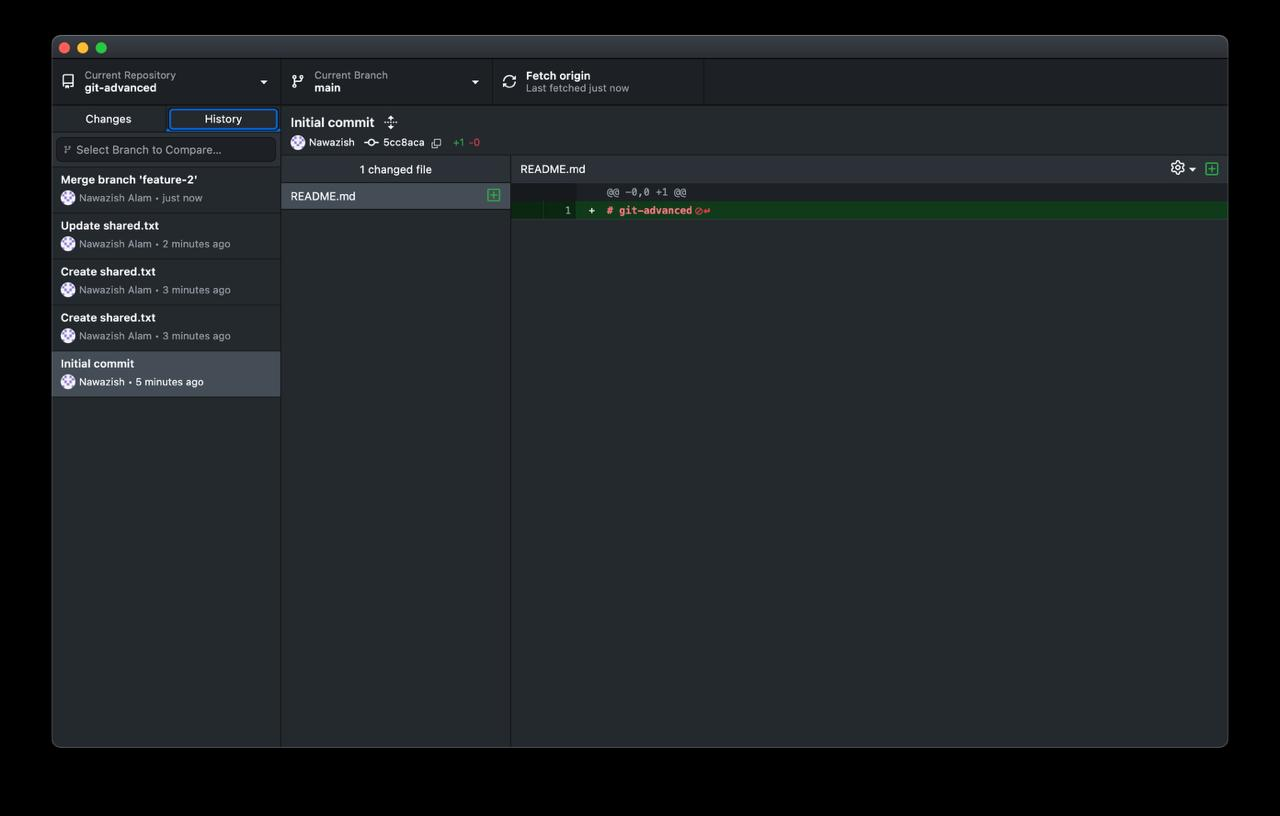
\includegraphics[width=0.8\linewidth]{commit.jpg} % Adjusted width
     \hspace{4 cm}
     \caption{Screenshot of the GitHub repository showing the initial commit history.}
\end{figure}

% Screenshot 2 
\begin{figure}[h!]
    \centering
    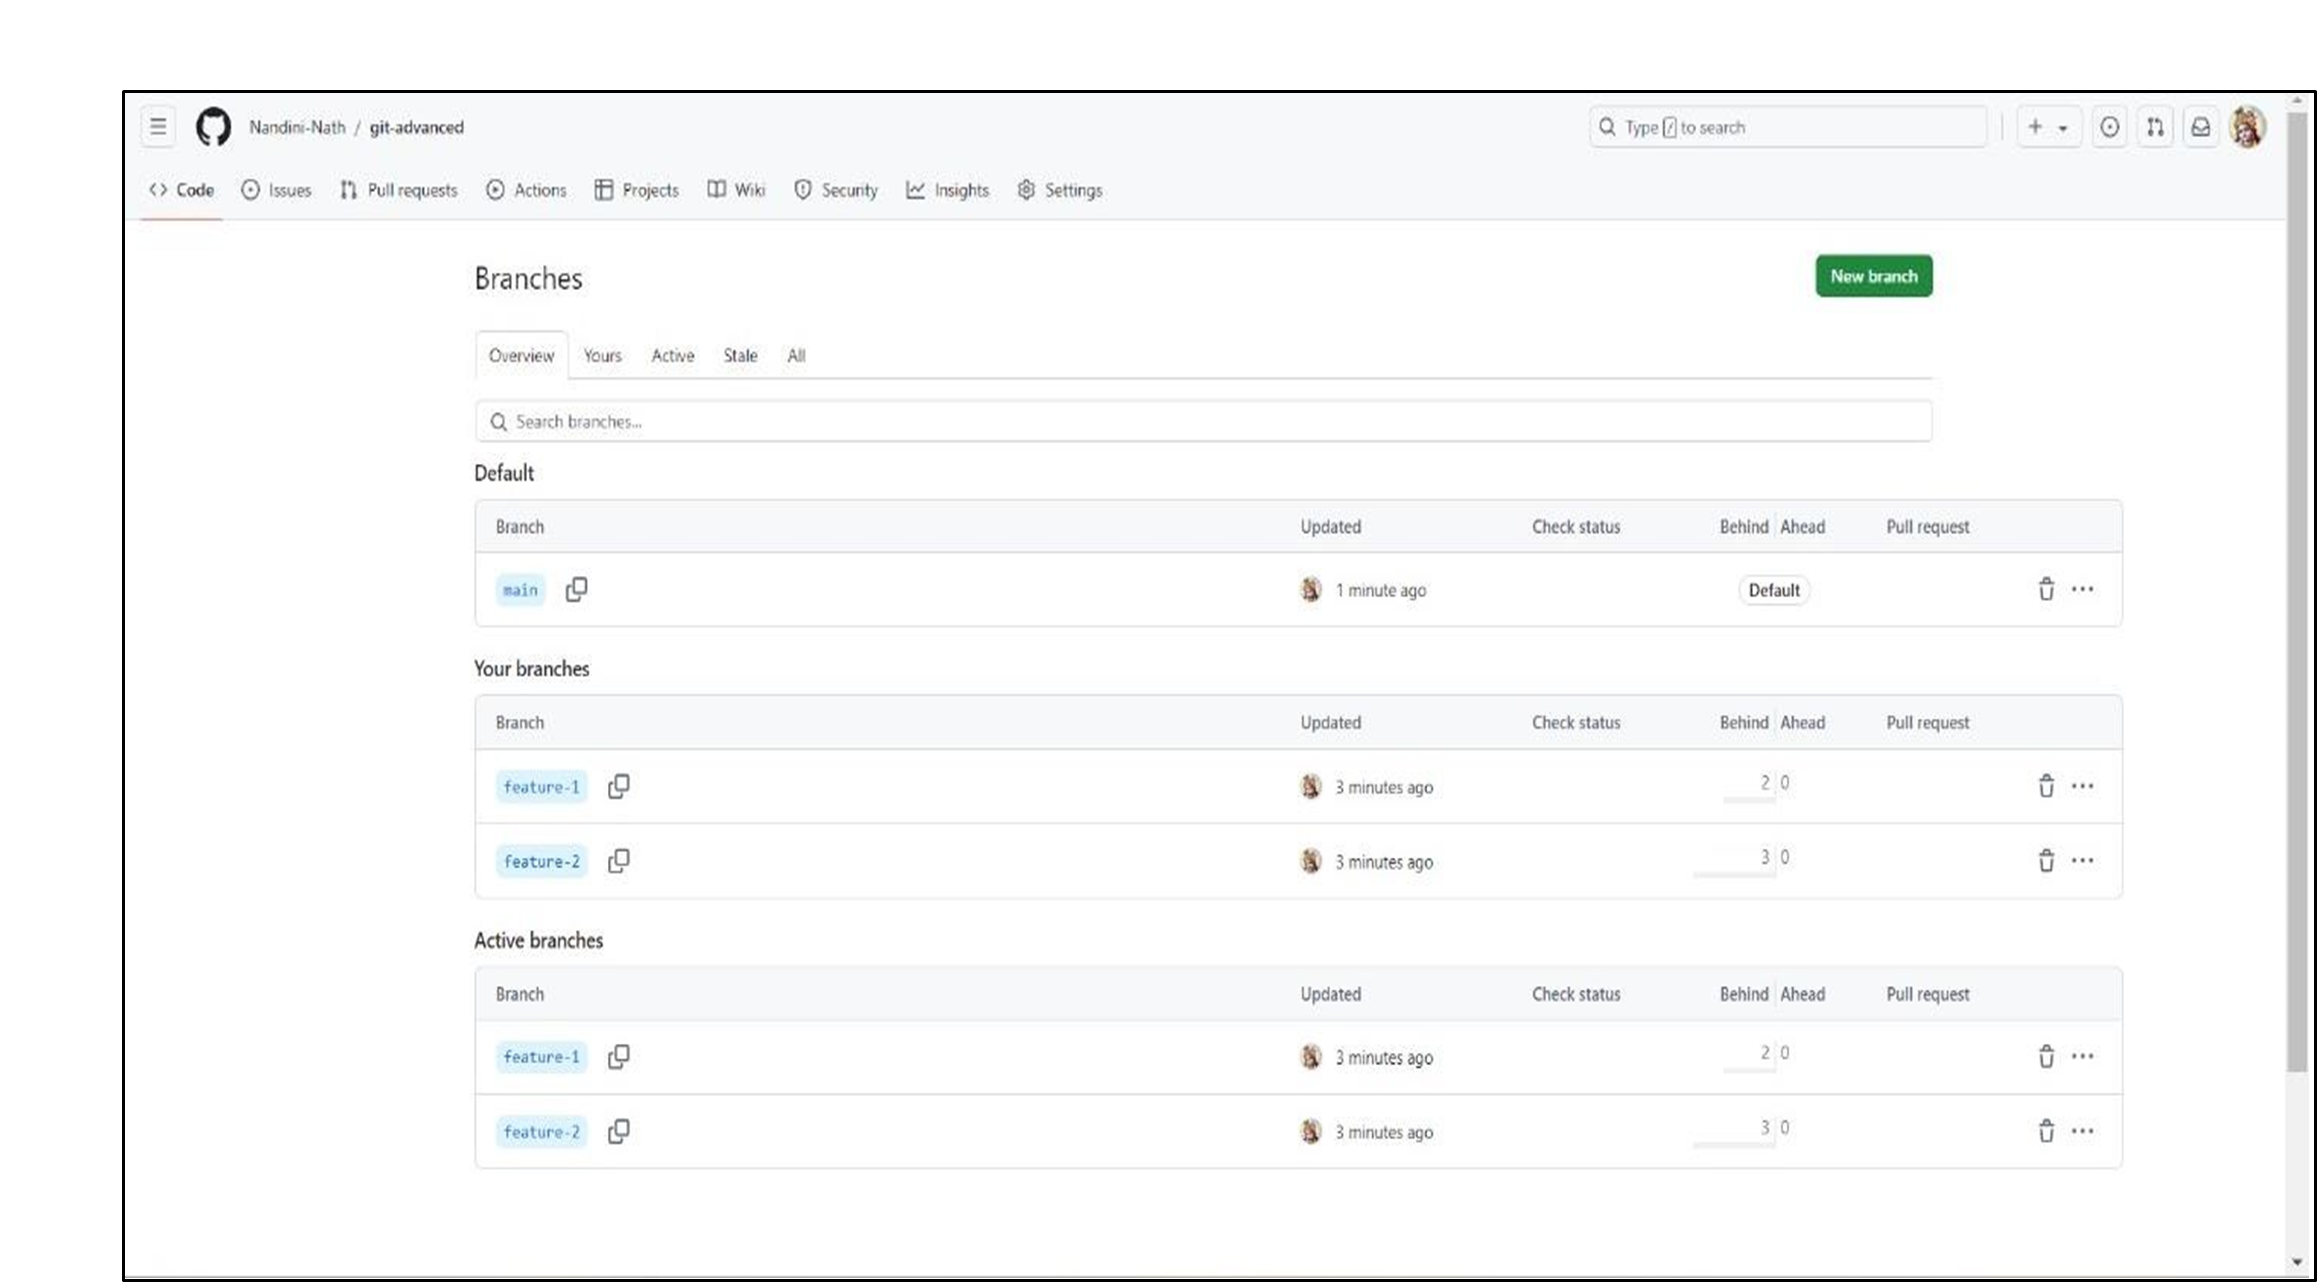
\includegraphics[width=0.8\linewidth]{branch.png} % Adjusted width
     \hspace{4 cm}
    \caption{Screenshot of the GitHub repository showing the branching.}
\end{figure}
\vspace{0 cm}

\newpage
\begin{tikzpicture}
    [remember picture, overlay]
    \draw[line width = 2pt, black] 
        ($(current page.north west) + (1cm,-1cm)$) 
        rectangle 
        ($(current page.south east) + (-1cm,1cm)$);
\end{tikzpicture}
\vspace{1 cm}
\begin{figure}[h!]
    \centering
    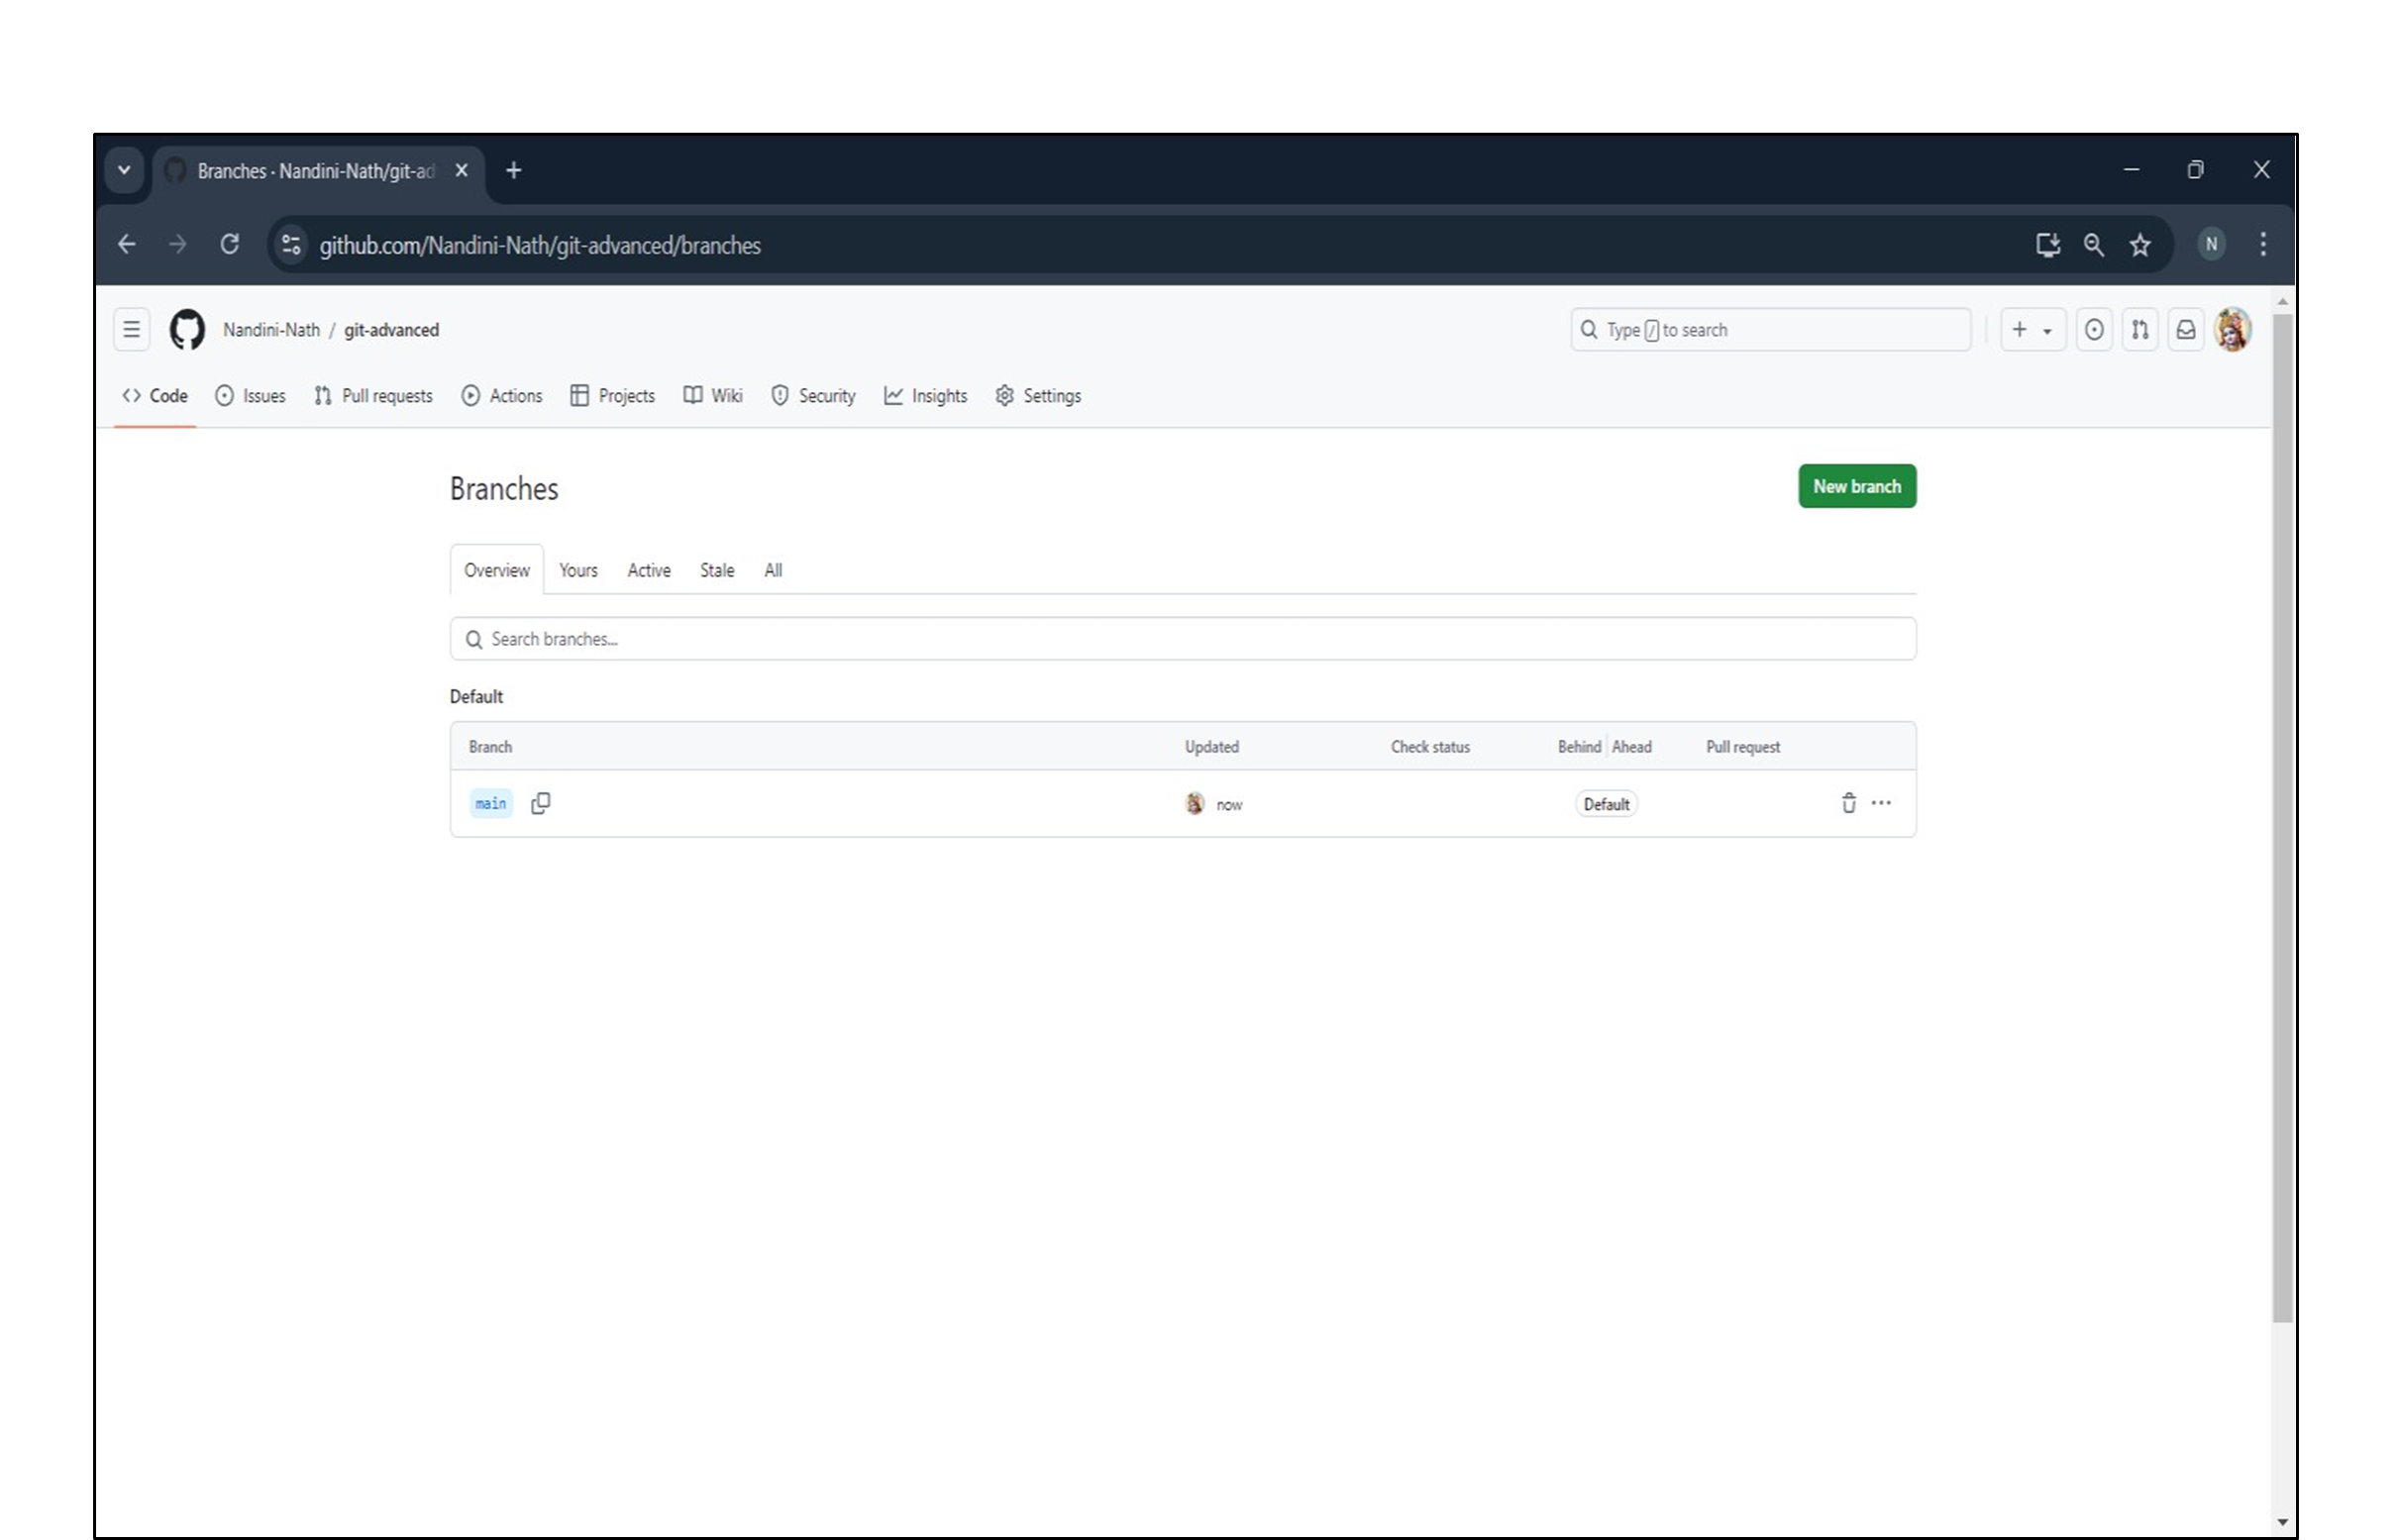
\includegraphics[width=0.8\linewidth]{delete.png}
    \hspace{4 cm}
    \caption{Repository after deleting branches `feature-1' and `feature-2'.}
    \label{fig:enter-label}
\end{figure}
% Screenshot 4
\hspace{6 cm}
\begin{figure}[h!]
    \centering
    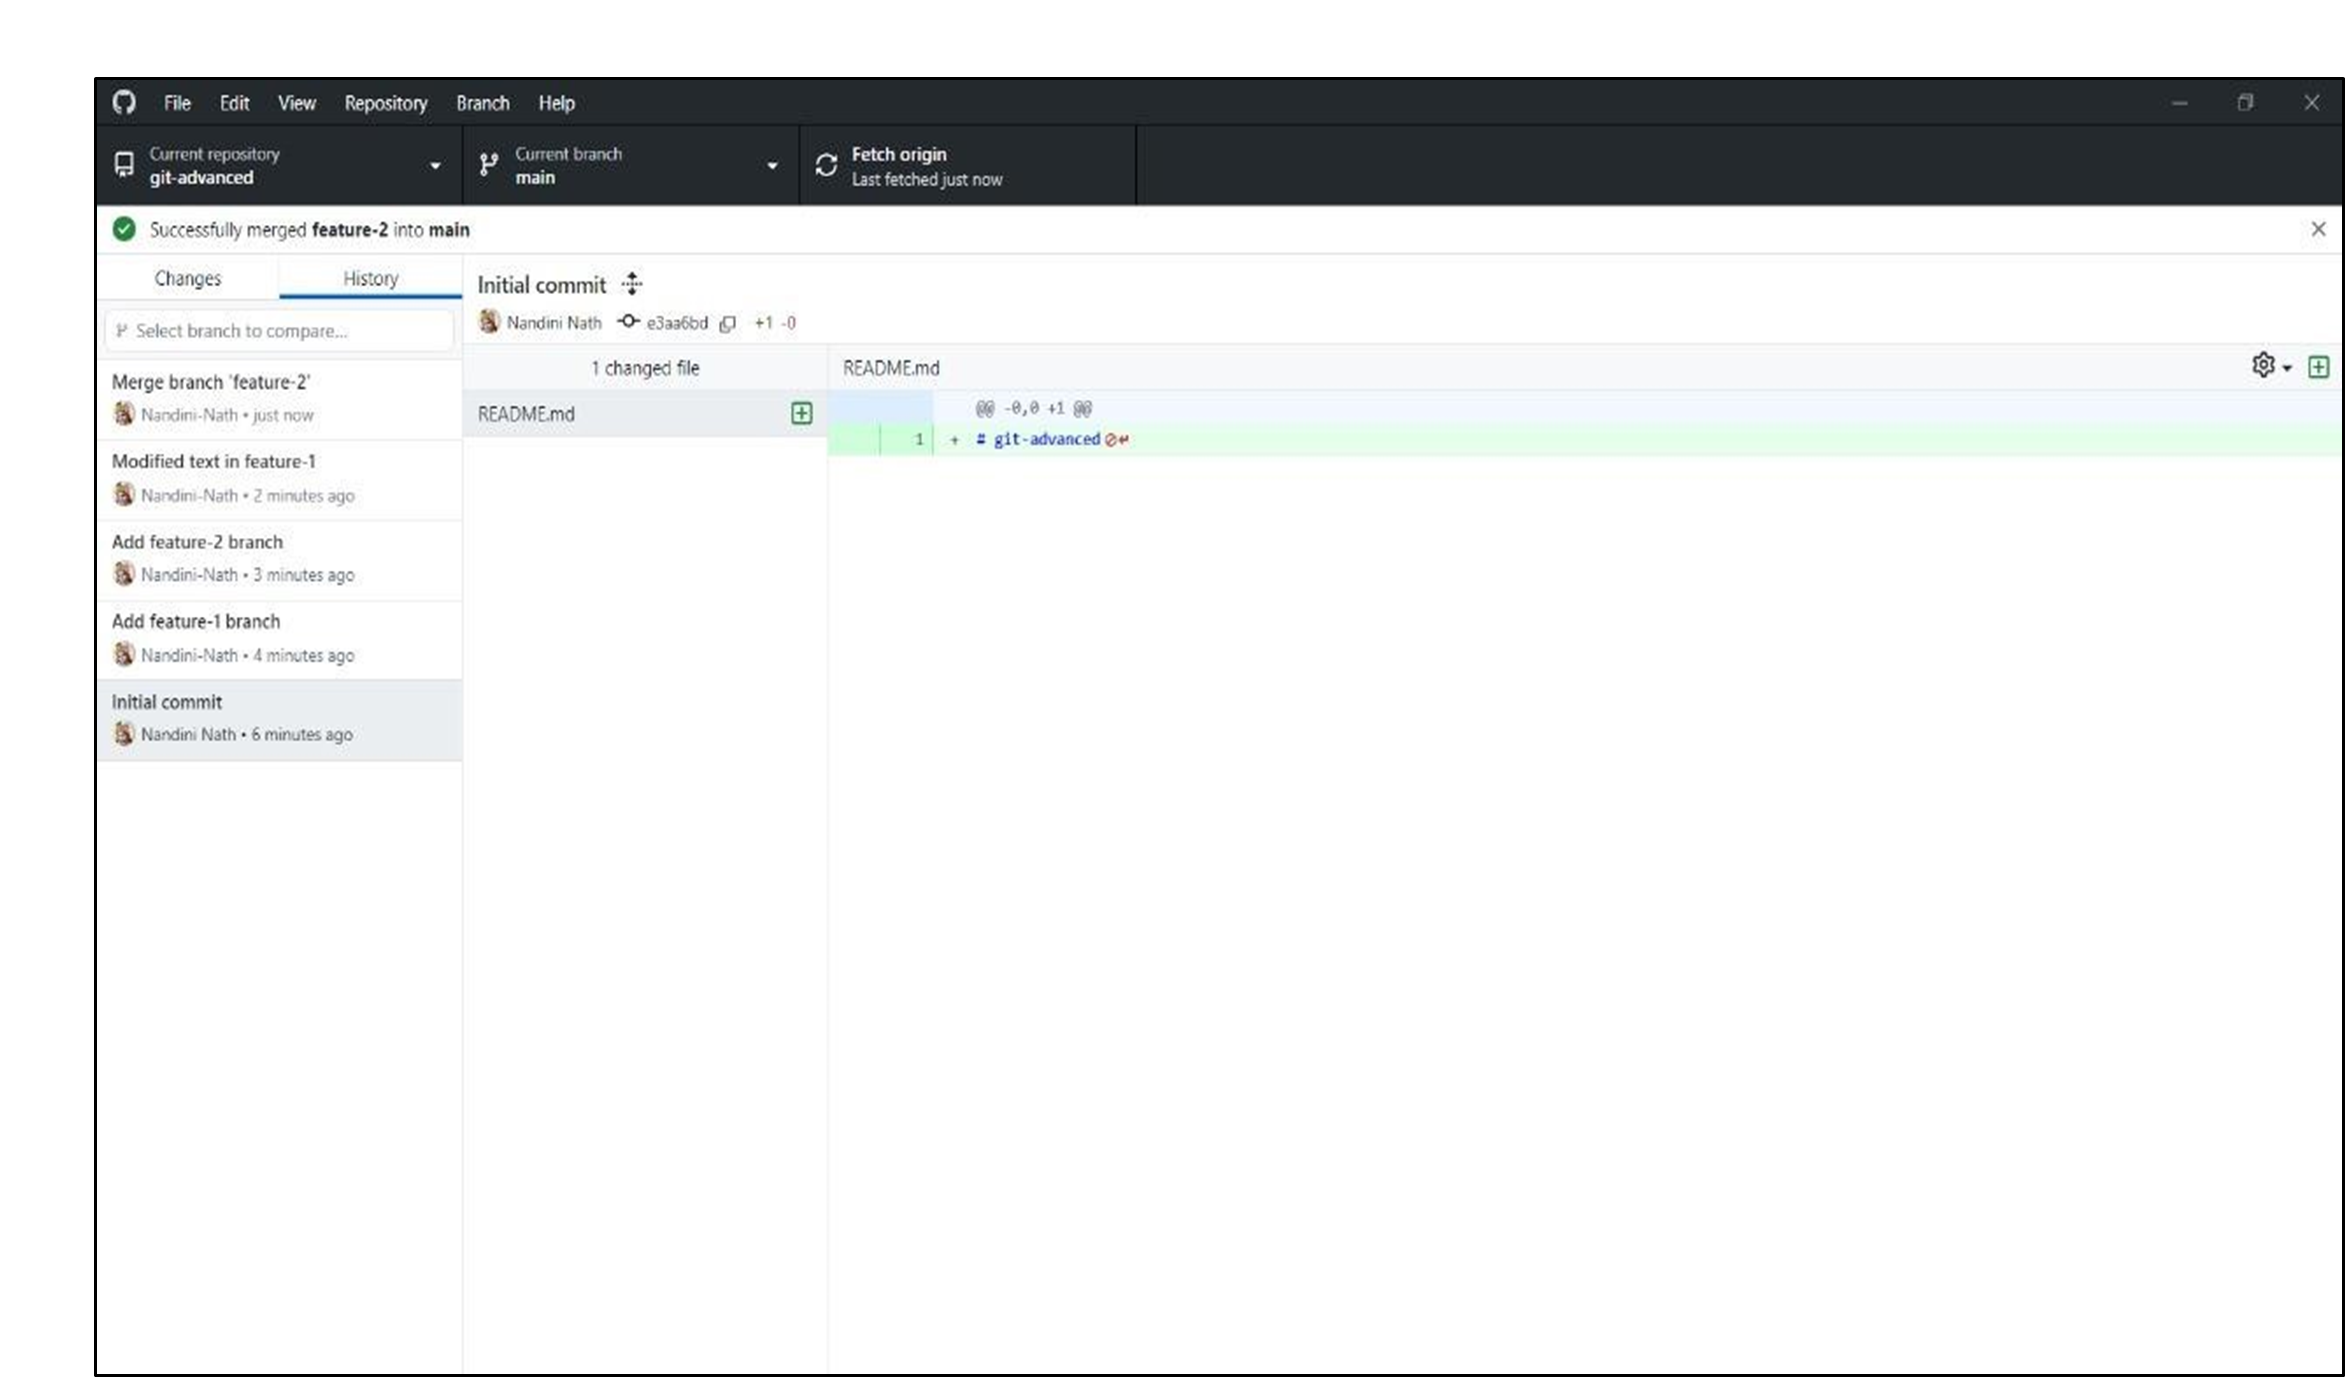
\includegraphics[width=0.8\linewidth]{gitlog.png} % Adjusted width
    \hspace{4 cm}
    \caption{Screenshot of the local machine showing the Git log.}
\end{figure}
\hspace{6 cm}
% Screenshot 5
\newpage
\begin{tikzpicture}
    [remember picture, overlay]
    \draw[line width = 2pt, black] 
        ($(current page.north west) + (1cm,-1cm)$) 
        rectangle 
        ($(current page.south east) + (-1cm,1cm)$);
\end{tikzpicture}
\vspace{-2cm}
\begin{figure}[h!]
    \centering
    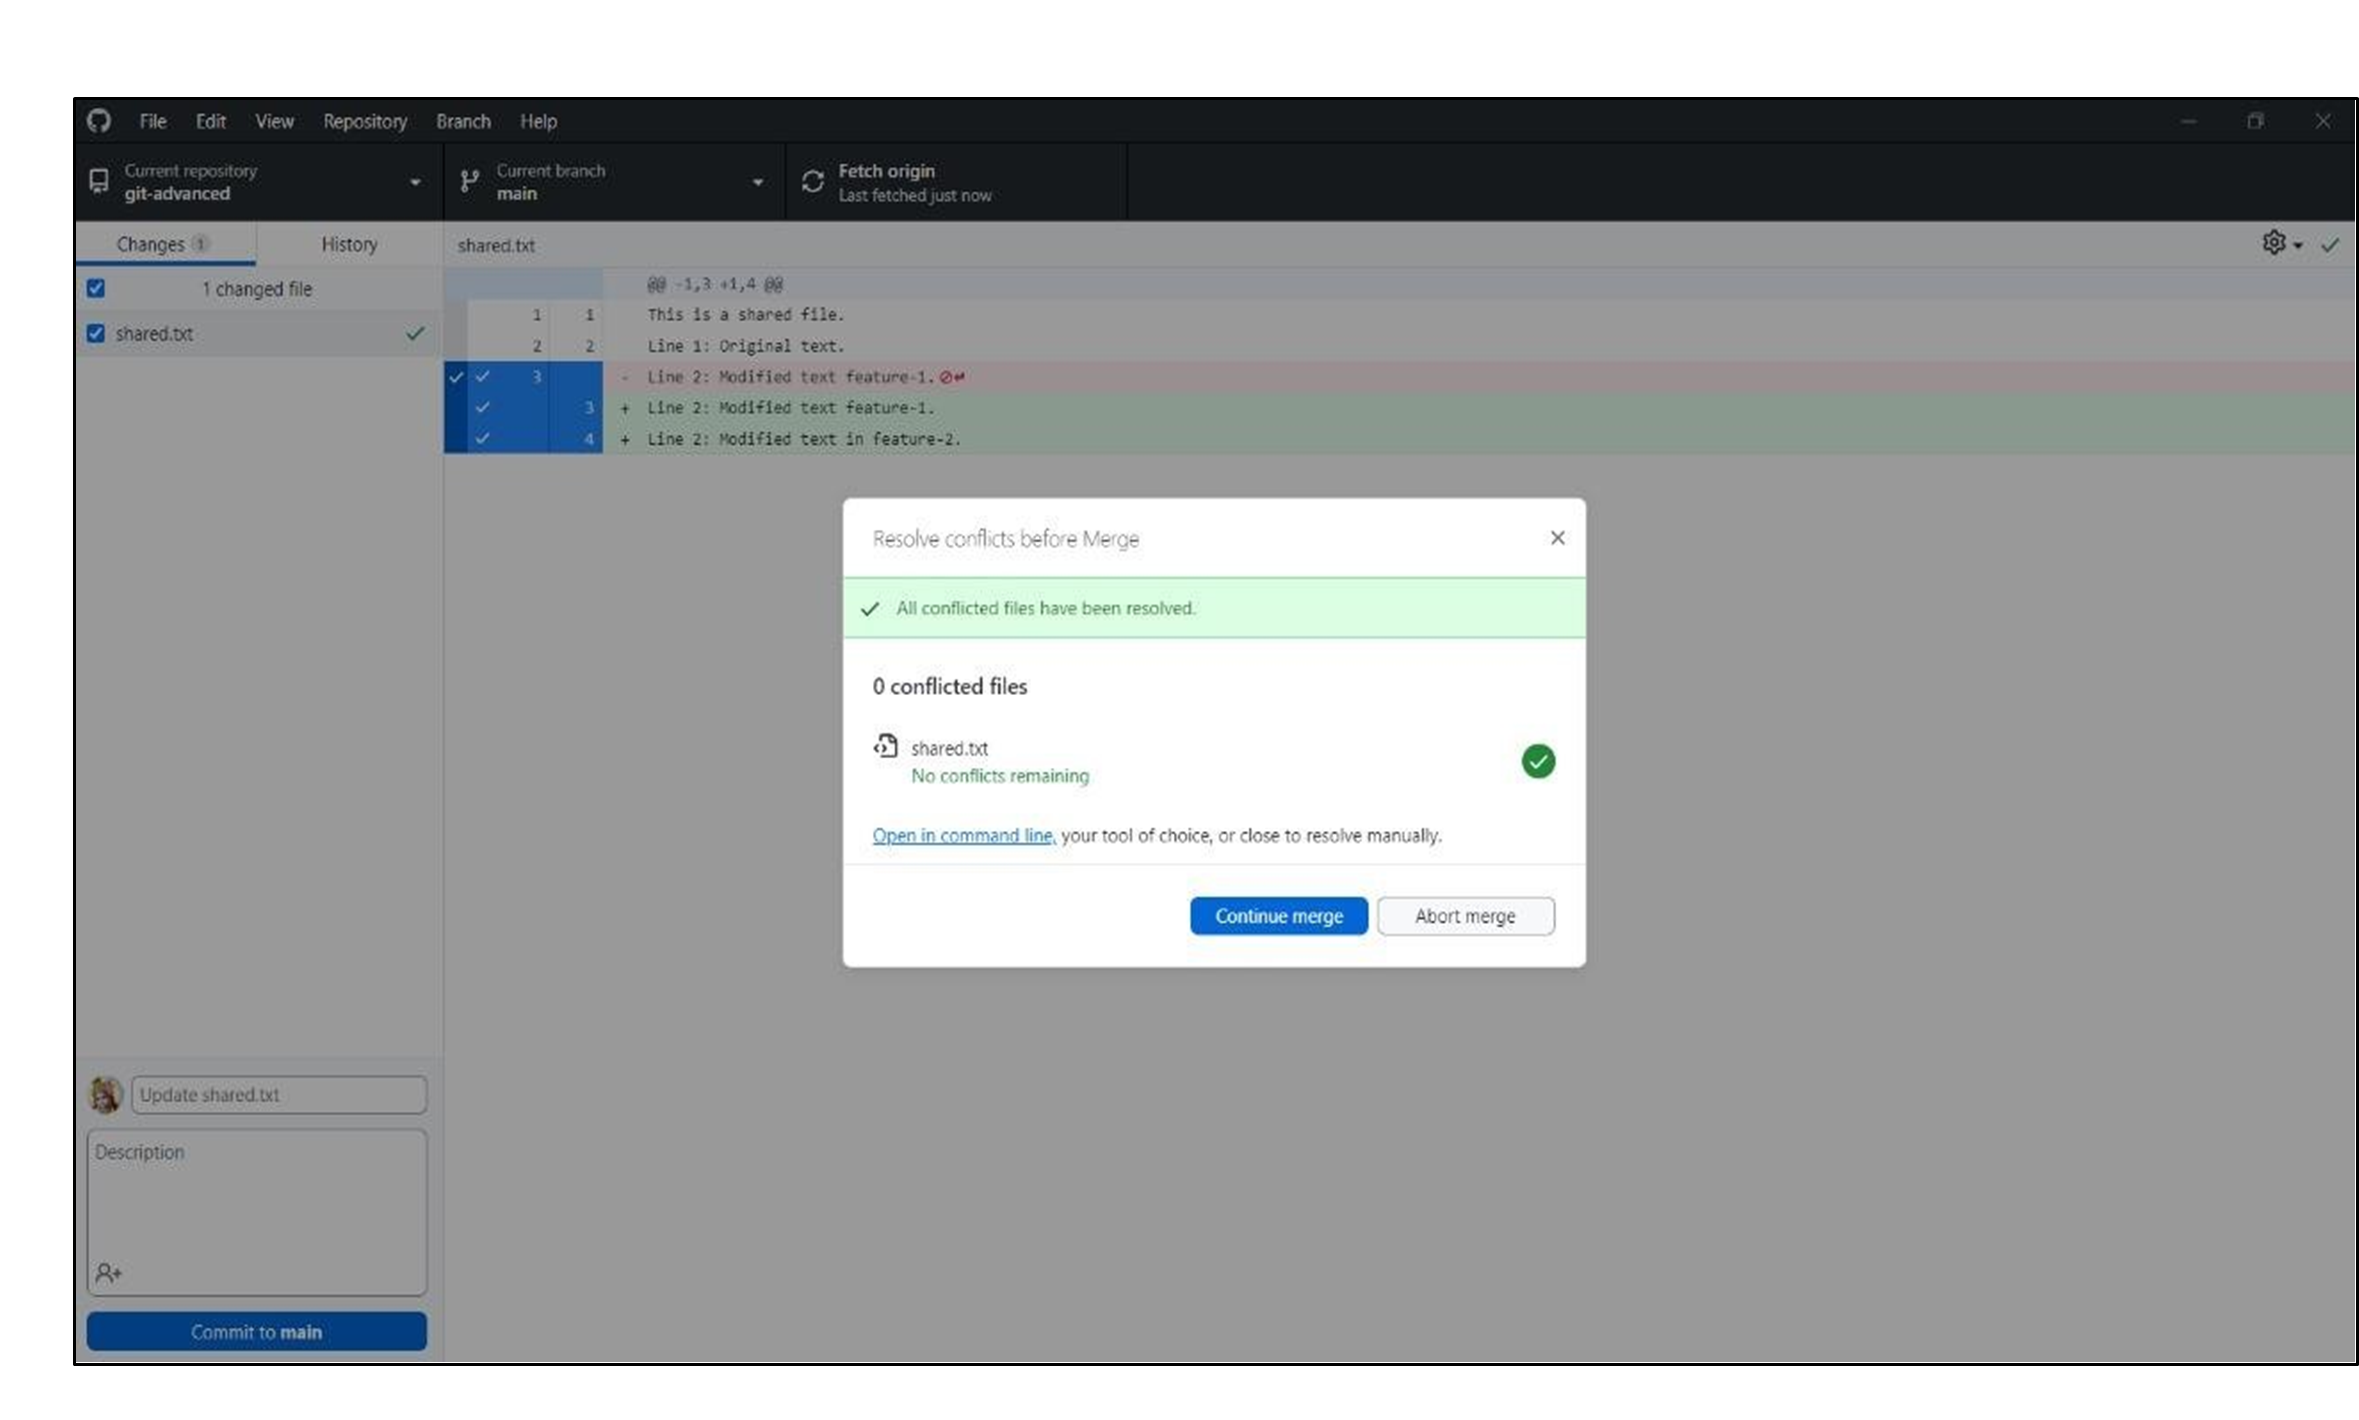
\includegraphics[width=0.8\linewidth]{conflict.png} % Adjusted width
    \hspace{4 cm}
    \caption{Screenshot of the local machine showing conflict resolution.}
\end{figure}

\subsection*{\LARGE{Write-Up: Experience with Git Branching {\underline{and Merging}}}}
\hspace{1 cm}
\paragraph{}
This assignment focused on the use of Git branching and merging to manage features in a collaborative environment. After creating separate branches for feature-1 and feature-2, each was developed independently.
When merging feature-1 into the main branch, there were no conflicts. However, the merge of feature-2 caused a conflict in the shared.txt file. Conflict resolution was done manually, ensuring that the changes from both branches were retained.
The practical experience highlighted the importance of clear commit messages and Git’s branching capabilities for parallel development and conflict management.

\newpage
\begin{tikzpicture}
    [remember picture, overlay]
    \draw[line width = 2pt, black] 
        ($(current page.north west) + (1cm,-1cm)$) 
        rectangle 
        ($(current page.south east) + (-1cm,1cm)$);
\end{tikzpicture}
\vspace{-2cm}
\subsection*{Entry by: Rajarshi Biswas}
\textit{Date: [\today]}\\

\newpage
\begin{tikzpicture}
    [remember picture, overlay]
    \draw[line width = 2pt, black] 
        ($(current page.north west) + (1cm,-1cm)$) 
        rectangle 
        ($(current page.south east) + (-1cm,1cm)$);
\end{tikzpicture}
\vspace{-2cm}
\subsection*{Entry by: Aabir Sengupta}
\textit{Date: [\today]}\\
\section*{\underline{{\Large{Assignment 6 : Make a CV using LaTeX}}}}
\vspace{0.5 cm}
\begin{flushleft}
    \textbf{\Large{\underline{Source code link:}}}$\href{https://github.com/Rajarshi-2005/LaTeX_Assignment_Group-11/blob/main/39959223039_BscForensic_Aabir.tex}{https://github.com/Rajarshi-2005/LaTeX_Assignment_Group-11/blob/main/39959223039_BscForensic_Aabir.tex}$
\end{flushleft}
\vspace{0.8 cm}
\begin{flushleft}
    \textbf{\underline{Output:}}
\end{flushleft}
\fbox{\includegraphics[width=0.8\linewidth]{cv.png}} % Adjusted width

\end{document}
